\documentclass[professionalfonts,compress,unicode]{beamer}

\usepackage{amsmath,amssymb}
\usepackage{empheq}
\usepackage[utf8]{inputenc}

\usepackage[russian]{babel}

\usepackage{ifthen}

\def\[#1\]{\begin{align*}#1\end{align*}}

\newcommand\myframe[3][dup]{
\ifthenelse{\equal{#1}{}}{}{\ifthenelse{\equal{#1}{dup}}{\subsection{#2}}{\subsection{#1}}}
\frame{\frametitle{#2}{#3}}%
}


\usetheme{Warsaw}
\usecolortheme{uranix}

\setbeamertemplate{headline}
{%
  \begin{beamercolorbox}[sep=0.3cm,wd=\paperwidth]{section in head/foot}%
    \usebeamerfont{frametitle}%
    \vbox{}\vskip-1ex%
    \strut\insertsectionhead\strut\par%
    \vskip-1ex%
  \end{beamercolorbox}%
}
\setbeamertemplate{navigation symbols}{}
\setbeamertemplate{footline}{}
\setbeamertemplate{caption}[numbered]

\renewcommand{\thefootnote}{\fnsymbol{footnote}}

\graphicspath{{images//}}

\title[Краевая задача]{Краевая задача для ОДУ\\ Жесткая краевая задача}
\author[Цыбулин И.В.]{Скалько Юрий Иванович\\
\textbf{Цыбулин Иван}
\\Шевченко Александр}
\date{}
%\vspace{0.3cm}

\begin{document}

{
\setbeamertemplate{headline}[default]
\frame{
\titlepage
}

%\frame{
%\frametitle{Содержание}
%\small
%%\tiny
%\tableofcontents
%}
}

\section{ }

%\myframe{Материалы по курсу вычислительной математики}
%{
%\begin{itemize}
	%\item 
		%Материалы курса (методички, лекции, учебники и др.) можно найти 
		%на сайте кафедры вычислительной математики
		%{\color{blue} http://crec.mipt.ru/study/materials/compmath/}
	%\item 
		%Любые вопросы по курсу (и не только) можно присылать на почтовый ящик
		%{\color{blue} tsybulinhome@gmail.com}
%\end{itemize}
%}

\def\L{\mathcal{L}}

\section{Краевая задача}
\myframe{Краевая задача для ОДУ 2го порядка}
{
	В отличие от задачи Коши, условия на функцию и производную ставятся на обоих концах отрезка
	\begin{empheq}[left=\empheqlbrace]{align*}
	&y''(x) = f(x, y(x), y'(x))\\
	&g(a,y(a),y'(a)) = 0\\
	&g(b,y(b),y'(b)) = 0
	\end{empheq}
	Требуется найти решение $y(x)$ при $x \in [a, b]$
}

\myframe{Линейная краевая задача для ОДУ 2го порядка}
{
	В линейном случае функции $f$ и $g$ линейно зависят от $y(x)$
	\begin{empheq}[left=\empheqlbrace]{align*}
	&\frac{d}{dx}\left[p(x)y'(x)\right] - q(x) y(x) = f(x)\\
	&\alpha_1 y(a) + \beta_1 y'(a) = \gamma_1\\
	&\alpha_2 y(b) + \beta_2 y'(b) = \gamma_2
	\end{empheq}
}

\myframe{Методы решения}
{
	\begin{itemize}
		\item Для линейных задач
		\begin{itemize}
			\item Метод численного построения общего решения
			\item Метод прогонки
		\end{itemize}
		\item Для нелинейных задач
		\begin{itemize}
			\item Метод стрельбы
			\item Метод линеаризации
		\end{itemize}
	\end{itemize}
}

\myframe{Метод численного построения общего решения}
{
	Линейность задачи позволяет искать решение в виде суммы частного решения неоднородной
	задачи и общего решения однородной. Для задачи второго порядка общее решение состоит из линейной комбинации двух
	линейно независимых решений
	\[
	y(x) = C_1 y_1(x) + C_2 y_2(x) + y_3(x)
	\]
	Здесь $y_1,y_2$ - линейно независимые решения однородной задачи, а $y_3$ - некоторое решение неоднородной.
}

\myframe[]{Метод численного построения общего решения}
{
	Для численного построения $y_1,y_2$ и $y_3$ можно решить 3 \emph{задачи Коши}.
	\begin{columns}[T]
	\begin{column}{0.6\textwidth}
	\begin{empheq}[left=\empheqlbrace]{align*}
		&\frac{d}{dx}\left[p(x)y_1(x)\right] - q(x) y_1(x) = 0\\
		&y_1(a) = 1\\
		&y_1'(a) = 0
	\end{empheq}	
	\end{column}
	\begin{column}{0.6\textwidth}
	\begin{empheq}[left=\empheqlbrace]{align*}
		&\frac{d}{dx}\left[p(x)y_2(x)\right] - q(x) y_2(x) = 0\\
		&y_2(a) = 0\\
		&y_2'(a) = 1
	\end{empheq}	
	\end{column}
	\end{columns}
	
	\begin{empheq}[left=\empheqlbrace]{align*}
		&\frac{d}{dx}\left[p(x)y_3(x)\right] - q(x) y_3(x) = f(x)\\
		&y_3(a) = 0\\
		&y_3'(a) = 0
	\end{empheq}	
}

\myframe[]{Метод численного построения общего решения}
{
	Коэффициенты $C_1, C_2$ в $y(x) = C_1 y_1(x) + C_2 y_2(x) + y(3)$ теперь находятся из линейной системы
	\begin{empheq}[left=\empheqlbrace]{align*}
		&\alpha_1 C_1 + \beta_1 C_2 = \gamma_1\\
		&\alpha_2 \Big(C_1 y_1(b) + C_2 y_2(b) + y_3(b)\Big) + \\
		&\beta_2 \Big(C_1 y_1'(b) + C_2 y_2'(b) + y_3'(b)\Big)  = \gamma_2
	\end{empheq}	
}

\myframe[]{Метод численного построения общего решения}
{
	Рассмотрим краевую задачу
	\begin{empheq}[left=\empheqlbrace]{align*}
	&y''(x) - 100 y(x) = 0\\
	&y(0) = 1\\
	&y(1) = 1
	\end{empheq}
	Соответствующие функции $y_1, y_2$ и $y_3$ будут
	\begin{columns}[T]
	\begin{column}{0.5\textwidth}
	\begin{empheq}[left=\empheqlbrace]{align*}
	y_1(x) &= \ch 10 x\\
	y_2(x) &= \frac{\sh 10 x}{10}\\
	y_3(x) &= 0
	\end{empheq}
	\end{column}
	\begin{column}{0.5\textwidth}
	\[
	& 
	\begin{pmatrix}
		1 & 0\\
		\ch 10 & \frac{\sh 10}{10}
	\end{pmatrix}
	\begin{pmatrix}
		C_1\\
		C_2
	\end{pmatrix}	= 
	\begin{pmatrix}
		1\\
		1
	\end{pmatrix}\\
	& \mu = \frac{\sh 10}{10} \approx 1100
	\]
	\end{column}
	\end{columns}
	Система плохо обусловлена, и $C_1$ и $C_2$ определяются с большой погрешностью
}

\myframe{Метод прогонки}
{
	Введем на отрезке $[a,b]$ сетку с шагом $h$. Рассмотрим разностную аппроксимацию краевой задачи
	\begin{empheq}[left=\empheqlbrace]{align*}
		&\frac{\left(p_{m+\frac{1}{2}}\frac{y_{m+1}-y_m}{h}\right)-\left(p_{m-\frac{1}{2}}\frac{y_m-y_{m-1}}{h}\right)}{h}
		-q_m y_m = f_m\\
		&\alpha_1 y_1 + \beta_1 \frac{y_2 - y_1}{h} = \gamma_1\\
		&\alpha_2 y_M + \beta_2 \frac{y_M - y_{M-1}}{h} = \gamma_2
	\end{empheq}	
	Это система линейных уравнений с $M$ неизвестными и $M$ уравнениями, причем в $m$-ом уравнении присутствуют только неизвестные 
	$y_{m-1},y_m,y_{m+1}$. Для этой трехдиагональной система можно применить метод прогонки
}

\myframe[]{Метод прогонки}
{
	Выпишем отдельно $m$-ое уравнение
	\[
	\frac{\left(p_{m+\frac{1}{2}}\frac{y_{m+1}-y_m}{h}\right)-\left(p_{m-\frac{1}{2}}\frac{y_m-y_{m-1}}{h}\right)}{h}
		-q_m y_m = f_m\\	
	\]
	
	\[
	p_{m-\frac{1}{2}}y_{m-1}-\left(p_{m-\frac{1}{2}}+p_{m-\frac{1}{2}}+q_m h^2\right)y_m+p_{m+\frac{1}{2}}y_{m+1} = f_m h^2
	\]
	Если $p>0$ и $q>0$, то на главной диагонали матрицы стоят элементы, по модулю превосходящие сумму модулей внедиагональных.
	Это условие диагонального преобладания достаточно для устойчивости прогонки.
}

\section{Нелинейная краевая задача}
\myframe{Метод стрельбы}
{
	Большинство методов для решения нелинейных краевых задач являются итерационными. Метод стрельбы на каждом шаге
	решает некоторую задачу Коши с целью ``попасть'' в правое граничное условие, корректируя начальные данные Коши.
}

\myframe[]{Метод стрельбы}
{
	Для задачи
	\begin{empheq}[left=\empheqlbrace]{align*}
		&y'' = f(x, y, y')\\
		&y(a) = y_0\\
		&y(b) = y_1
	\end{empheq}	
	будем решать задачу Коши с параметром $\alpha$
	\begin{empheq}[left=\empheqlbrace]{align*}
		&y_{\alpha}'' = f(x, y_{\alpha}, y_{\alpha}')\\
		&y_{\alpha}(a) = y_0\\
		&y_{\alpha}'(a) = \tg \alpha
	\end{empheq}
	Требуется решить уравнение $y_{\alpha}(b) = y_1$ относительно $\alpha$. 
	Это можно сделать, например, методом секущих. Но необходимо помнить, что
	каждое вычисление $y_{\alpha}(b)$ 
	стоит одного решения задачи Коши.
}

\myframe{Метод линеаризации}
{
	Метод линеаризации позволяет решать нелинейную краевую задачу последовательно решая 
	вспомогательные \emph{линейные}	задачи.
	
	Так же, как в случае нелинейных алгебраических уравнений, когда нелинейная функция
	в точке заменялась ее линейным приближением, нелинейная краевая задача заменяется 
	линейной в окрестности приближенного решения.
	
	\[
	&f(x,y,y') = f(x,\tilde{y},\tilde{y}') + f_y(x,\tilde{y},\tilde{y}')(y-\tilde{y}) + f_{y'}(x,\tilde{y},\tilde{y}')(y'-\tilde{y}')\\
	\]
	Аналогично, можно разложить и граничные условия
}

\myframe[]{Метод линеаризации}
{
	Предположим, что имеется некоторое приближение $\tilde{y}(x)$, которое удовлетворяет граничным условиям.
	Будем искать решение в виде $y(x) = \tilde{y}(x) + v(x)$. Предположим, что $v$ - малая поправка.
	
	\begin{empheq}[left=\empheqlbrace]{align*}
		&v'' = f_y(x,\tilde{y},\tilde{y}')v + f_{y'}(x,\tilde{y},\tilde{y}')v'\\
		&g_y(a,\tilde{y}(a),\tilde{y}'(a))v(a) + g_y(a,\tilde{y}(a),\tilde{y}'(a))v'(a) = 0\\
		&g_y(b,\tilde{y}(b),\tilde{y}'(b))v(b) + g_y(b,\tilde{y}(b),\tilde{y}'(b))v'(b) = 0
	\end{empheq}
	
	Решив эту линейную систему, получаем $\tilde{\tilde{y}}(x) = \tilde{y}(x) + v(x)$ - новое приближение.
}

\section{Краевая задача для СОДУ}
\myframe{Краевая задача для СОДУ} 
{
	Рассмотрим краевую задачу для систем ОДУ 1го порядка
	\begin{empheq}[left=\empheqlbrace]{align*}
		&\frac{dy(x)}{dx} = A(x)y(x) + f(x)\\
		&G_jy(a) = g_j, j=\overline{1,k}\\
		&G_jy(b) = g_j, j=\overline{k+1,n}
	\end{empheq}
	
	$k$ граничных условий задано на левом конце, $n-k$ на правом
}

\myframe{Жесткая краевая задача}
{
	Краевая задача называется жесткой, если спектр матрицы $A(x)$ разбивается на $3$ области
	\begin{itemize}
		\item Мягкий спектр: $|\lambda| < \ell$\\
		\item Жесткий положительный спектр: $\operatorname{Re}(\lambda) > L$
		\item Жесткий отрицательный спектр: $\operatorname{Re}(\lambda) < -L$
	\end{itemize}
	при $L \gg \ell$
	\begin{figure}%
	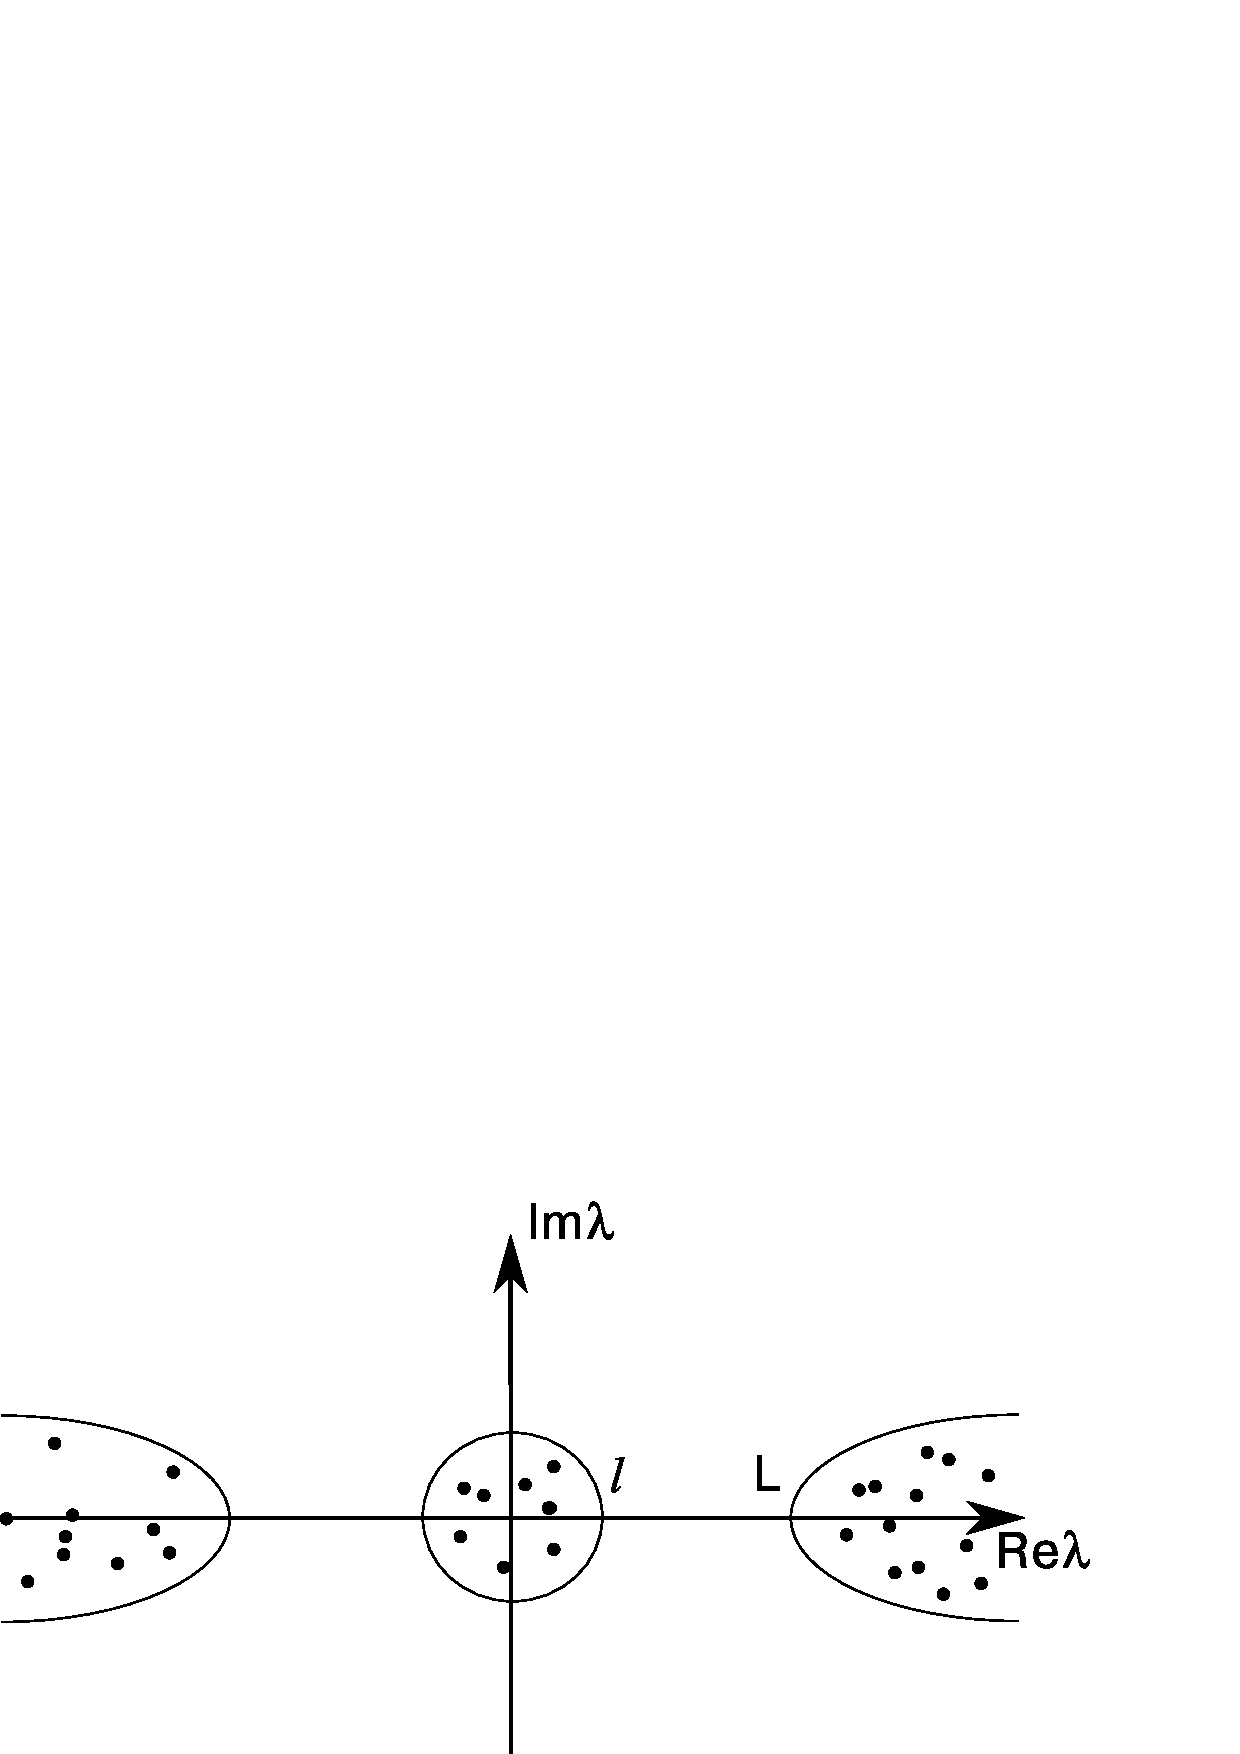
\includegraphics[width=0.8\columnwidth]{stiff.pdf}%
	\end{figure}
}

\myframe[]{Жесткая краевая задача}
{
	Решение краевой задачи - некоторая линейная комбинация решений с различными $\lambda$, причем
	решения с $\lambda$ из
	\begin{itemize}
		\item мягкого спектра - небольшие по модулю
		\item жесткого положительного спектра - резко убывают влево
		\item жесткого отрициательного спектра - резко убывают вправо
	\end{itemize}
}

\myframe{Граничные условия для жесткой краевой задачи}
{
	Пусть в жесткой отрицательной части спектра находится $I_-$ собственных значений, причем это число больше числа граничных условий слева $k$.
	Решения из жесткой отрицательной части спектра быстро убывают вправо, и на правом конце по модулю очень малы (в $e^{LT}$ раз меньше чем на левом).
	Из-за этого, их вклад в граничные уравнения на правом конце практически нулевой (порядка ошибок округления). 
	
	Изменение коэффициентов при этих решениях практически не повлияет на правые граничные условия, поэтому коэффициенты можно надежно найти только из левых граничных
	условий. А левых граничных условий недостаточно, чтобы найти все коэффициенты при убывающих вправо решениях.
}

\myframe[]{Граничные условия для жесткой краевой задачи}
{
	Итак, чтобы задача была \emph{вычислительно корректной} требуется чтобы число условий слева было не меньше убывающих вправо решений, и, наоборот,
	число условий справа было не меньше числа убывающих влево решений.
}
%%%%%%%%%%%%%%%%%%%%%%%%%%%%%%%%%%%%%%%%%%%%%%%
%%%%%%%%%%%%%%%%%%%%%%%%%%%%%%%%%%%%%%%%%%%%%%%
%%%%%%%%%                            %%%%%%%%%%
%%%%%%%%%%%%%%%%%%%%%%%%%%%%%%%%%%%%%%%%%%%%%%%
%%%%%%%%%%%%%%%%%%%%%%%%%%%%%%%%%%%%%%%%%%%%%%%
{
\setbeamertemplate{headline}[default] 
\frame{
	\begin{center}
	{\Huge Спасибо за внимание!}
	\end{center}
	\bigskip
	\begin{center}
	{\color{blue}{tsybulinhome@gmail.com}}
	\end{center}
	}
}

\end{document}
